\documentclass[11pt,a4paper]{article}

% --- Packages ---
\usepackage[utf8]{inputenc}
\usepackage[margin=1in]{geometry}
\usepackage{amsmath,amssymb}
\usepackage{booktabs}
\usepackage{listings}
\usepackage{xcolor}
\usepackage{hyperref}
\usepackage{enumitem}
\usepackage{tikz}
\usetikzlibrary{shapes.geometric, arrows.meta, positioning, calc}

% --- Hyperlink Settings ---
\hypersetup{
    colorlinks=true,
    linkcolor=blue!70!black,
    citecolor=blue!70!black,
    urlcolor=blue!70!black
}

% --- Color Palette ---
\definecolor{codegreen}{rgb}{0.1,0.55,0.2}
\definecolor{codegray}{rgb}{0.45,0.45,0.45}
\definecolor{codepurple}{rgb}{0.5,0.1,0.7}
\definecolor{backcolour}{rgb}{0.97,0.97,0.98}
\definecolor{codeblue}{rgb}{0.13,0.29,0.53}

% --- Listings / Language Definition ---
\lstdefinelanguage{Rust}{
    keywords={as, break, const, continue, crate, else, enum, extern, false, fn, for, if, impl, in, let, loop, match, mod, move, mut, pub, ref, return, self, Self, static, struct, super, trait, true, type, unsafe, use, where, while, async, await, dyn, try, union},
    sensitive=true,
    morecomment=[l]{//},
    morecomment=[s]{/*}{*/},
    morestring=[b]",
    morestring=[b]'
}

% --- Listings / Code Styling ---
\lstdefinestyle{ruststyle}{
    language=Rust,
    backgroundcolor=\color{backcolour},
    commentstyle=\color{codegreen},
    keywordstyle=\color{codeblue}\bfseries,
    numberstyle=\tiny\color{codegray},
    stringstyle=\color{codepurple},
    basicstyle=\ttfamily\footnotesize,
    breakatwhitespace=false,
    breaklines=true,
    captionpos=b,
    keepspaces=true,
    numbers=left,
    numbersep=6pt,
    showspaces=false,
    showstringspaces=false,
    showtabs=false,
    tabsize=4,
    frame=single,
    rulecolor=\color{black!15}
}

\lstdefinestyle{bashstyle}{
    backgroundcolor=\color{backcolour},
    basicstyle=\ttfamily\footnotesize,
    breaklines=true,
    frame=single,
    rulecolor=\color{black!15}
}

\lstset{style=ruststyle}

\title{\textbf{Concat Rust (\texttt{grab}) \\ System Architecture \& Engineering Design Specification}}
\author{\textbf{System Engineering Team}}
\date{August 2026}

\begin{document}

\maketitle

\begin{abstract}
This document provides the formal architectural and algorithmic specification for \textbf{Concat Rust} (\texttt{grab}), a high-throughput code indexing daemon and accompanying CLI utility designed for LLM-assisted software engineering. The system condenses multi-repository codebases into high-density abstract syntax tree (AST) signature skeletons annotated with deterministic content hashes and line-of-code metrics. It maintains an incremental synchronization mirror, provides sub-millisecond AST and whole-file retrieval via an embedded HTTP daemon, and executes an optimized context-handshake protocol with downstream AI agents.
\end{abstract}

\tableofcontents
\newpage

% -----------------------------------------------------------------------------
\section{Executive Summary \& System Objectives}
% -----------------------------------------------------------------------------
LLM context windows, while expanding in capacity, suffer from quadratic attention degradation and cost bottlenecks when processing large repositories. Existing solutions either summarize code destructively (losing critical type signatures) or inject raw file dumps.

\textbf{Concat Rust} implements a deterministic, lossless structural compression scheme:
\begin{enumerate}[leftmargin=*]
    \item \textbf{AST Skeleton Extraction:} Compresses Rust and Go source files by stripping function, method, and macro implementation bodies while preserving top-level signatures, traits, structs, and module hierarchies.
    \item \textbf{Deterministic Body Hashing:} Replaces AST bodies with a unique 12-character lowercase hexadecimal hash computed via $\text{SHA-256}(\text{file\_path} \parallel \texttt{"\textbackslash n"} \parallel \text{body\_content})$.
    \item \textbf{Incremental Mirroring Engine:} Observes source directories, skipping build artifacts and binary blobs, and replicates active source states to a centralized working directory with nanosecond timestamp diffing.
    \item \textbf{Zero-Latency On-Demand Expansion:} Provides a local HTTP daemon and a command-line interface (\texttt{cli}) enabling AI agents to fetch individual AST bodies or full file contents in a single multi-target query.
\end{enumerate}

% -----------------------------------------------------------------------------
\section{System Architecture \& Component Topology}
% -----------------------------------------------------------------------------

\begin{figure}[htbp]
\centering
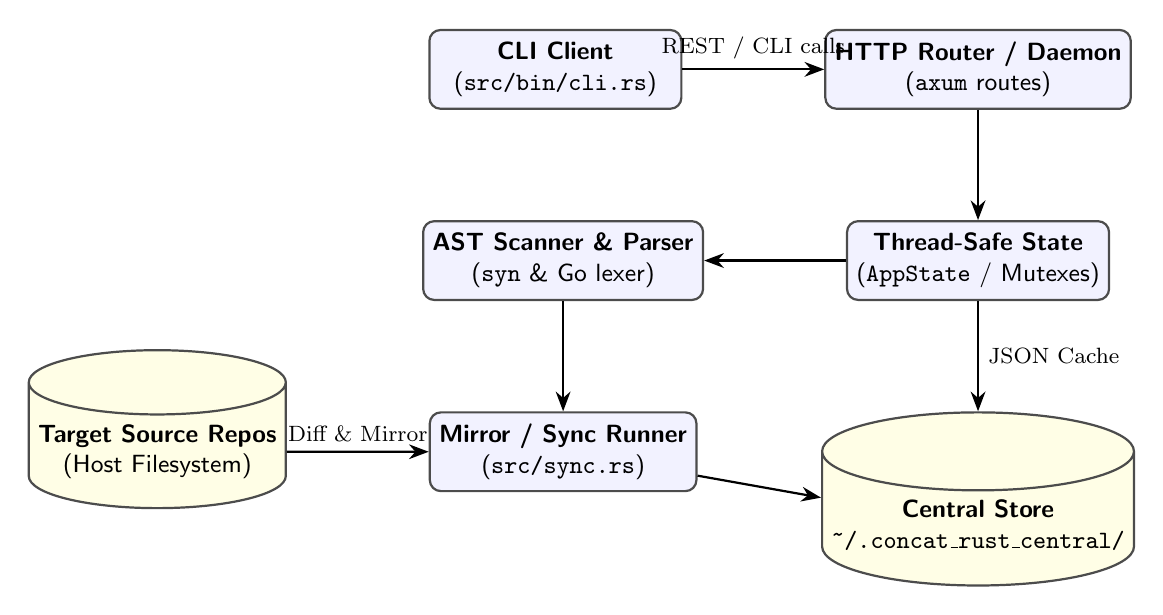
\begin{tikzpicture}[
    node distance=1.4cm and 1.8cm,
    block/.style={rectangle, draw=black!70, fill=blue!5, thick, rounded corners, minimum height=1cm, minimum width=3.2cm, align=center, font=\small\sffamily},
    storage/.style={cylinder, draw=black!70, fill=yellow!10, shape border rotate=90, aspect=0.25, thick, minimum height=1.2cm, minimum width=2.8cm, align=center, font=\small\sffamily},
    line/.style={-{Stealth[length=2.5mm]}, thick}
]

% Nodes
\node[block] (cli) {\textbf{CLI Client} \\ (\texttt{src/bin/cli.rs})};
\node[block, right=of cli] (http) {\textbf{HTTP Router / Daemon} \\ (\texttt{axum} routes)};
\node[block, below=of http] (state) {\textbf{Thread-Safe State} \\ (\texttt{AppState} / Mutexes)};
\node[block, left=of state] (scanner) {\textbf{AST Scanner \& Parser} \\ (\texttt{syn} \& Go lexer)};
\node[block, below=of scanner] (sync) {\textbf{Mirror / Sync Runner} \\ (\texttt{src/sync.rs})};
\node[storage, below=of state] (central) {\textbf{Central Store} \\ \texttt{\textasciitilde/.concat\_rust\_central/}};
\node[storage, left=of sync] (source) {\textbf{Target Source Repos} \\ (Host Filesystem)};

% Connections
\draw[line] (cli) -- node[above, font=\footnotesize] {REST / CLI calls} (http);
\draw[line] (http) -- (state);
\draw[line] (state) -- (scanner);
\draw[line] (scanner) -- (sync);
\draw[line] (sync) -- (central);
\draw[line] (source) -- node[above, font=\footnotesize] {Diff \& Mirror} (sync);
\draw[line] (state) -- node[right, font=\footnotesize] {JSON Cache} (central);

\end{tikzpicture}
\caption{Concat Rust High-Level Architectural Flow}
\label{fig:arch}
\end{figure}

% -----------------------------------------------------------------------------
\section{Formal Data Models \& Storage Layout}
% -----------------------------------------------------------------------------

\subsection{Repository Registry Data Model}
The repository registry (\texttt{src/registry.rs}) tracks registered source paths and mirror metadata.

\begin{lstlisting}[language=Rust, caption={Repository Registry Model}]
#[derive(Serialize, Deserialize, Clone, Debug)]
pub struct RepoEntry {
    pub id: String,                 // Slug identifier (e.g., "core-api")
    pub source_path: PathBuf,       // Host system absolute source path
    pub active: bool,               // Active filter status
    pub last_sync: Option<u64>,     // Epoch timestamp in seconds
    pub git_branch: Option<String>, // Active git branch name
    pub file_count: Option<usize>,  // Total indexed files
}

#[derive(Serialize, Deserialize, Clone, Debug, Default)]
pub struct RepoRegistry {
    pub repos: HashMap<String, RepoEntry>,
    pub central_dir: PathBuf,
}
\end{lstlisting}

\subsection{Daemon Cache \& Fingerprint Schema}
The cache (\texttt{src/cache.rs}) provides in-memory indexing of pre-parsed files, extracted AST bodies, usage counters, and pre-rendered skeleton segments.

\begin{lstlisting}[language=Rust, caption={Daemon Cache and AST Metadata Schema}]
#[derive(Serialize, Deserialize, Clone, Debug, PartialEq)]
pub struct FileFingerprint {
    pub mtime_nanos: u128,
    pub byte_size: u64,
    pub content_hash: String,       // SHA-256 over raw file payload
}

#[derive(Serialize, Deserialize, Clone, Debug)]
pub struct BodyMeta {
    pub filepath: String,
    pub loc: usize,
    pub byte_size: usize,
}

#[derive(Serialize, Deserialize, Clone, Debug)]
pub struct BodyEntry {
    pub meta: BodyMeta,
    pub body: String,               // Isolated original AST block text
}

#[derive(Serialize, Deserialize, Clone, Debug)]
pub struct FileEntry {
    pub loc: usize,
    pub byte_size: usize,
    pub body_hashes: Vec<String>,   // List of 12-char SHA-256 body hashes
    pub code: String,               // Formatted/Sanitized source
}

#[derive(Serialize, Deserialize, Clone, Debug, Default)]
pub struct DaemonCache {
    pub bodies: HashMap<String, BodyEntry>,
    pub files: HashMap<String, FileEntry>,
    pub skeleton_segments: HashMap<String, String>,
    pub file_order: Vec<String>,
    pub fingerprints: HashMap<String, FileFingerprint>,
    pub meta_prompt: String,
    pub generation: u64,
    pub file_hits: HashMap<String, u64>,
    pub hash_hits: HashMap<String, u64>,
    #[serde(skip)]
    pub cache_path: String,
}
\end{lstlisting}

\subsection{Disk Layout Hierarchy}
All internal states, mirror directories, and cache snapshots reside in a deterministic directory layout:
\begin{lstlisting}[style=bashstyle]
~/.concat_rust_central/
|-- .registry.json            # Serialized RepoRegistry
|-- .active_repo              # Plaintext string containing active repo ID
|-- concat_rust.cache.json    # Serialized DaemonCache
|-- <repo_id_1>/              # Exact mirror of repo 1 source files
|   |-- Cargo.toml
|   `-- src/
|       `-- main.rs
`-- <repo_id_2>/              # Exact mirror of repo 2 source files
    |-- go.mod
    `-- main.go
\end{lstlisting}

% -----------------------------------------------------------------------------
\section{AST Parsing, Hashing, \& Compression Pipelines}
% -----------------------------------------------------------------------------

\subsection{Stable Hash Construction Algorithm}
Hashes are deterministic across platforms and execution environments. Given an AST node string $B$ and relative file path $P$:
\begin{equation}
\mathcal{H}_{\text{body}}(B, P) = \text{SubStr}_{0, 12}\Big(\text{SHA256}\big(P \parallel \texttt{"\textbackslash n"} \parallel B\big)\Big)
\end{equation}
\begin{equation}
\mathcal{H}_{\text{file}}(C) = \text{SubStr}_{0, 12}\Big(\text{SHA256}\big(C\big)\Big)
\end{equation}
where $\text{SubStr}_{0, 12}$ yields the first 12 lower-case hex characters.

\subsection{Rust AST Compression Engine (\texorpdfstring{\texttt{src/compress.rs}}{src/compress.rs})}
Rust parsing uses `\texttt{syn}` to traverse the AST:
\begin{itemize}[leftmargin=*]
    \item \textbf{Functions (\texttt{Item::Fn}):} Body block extracted via line/column span slicing against raw source. Body is stored in \texttt{DaemonCache.bodies}, replaced in skeleton by:
    \begin{center}
    \texttt{\{ /* HASH:<hash> [<loc> LOC] */ \}}
    \end{center}
    \item \textbf{Implementation Blocks (\texttt{Item::Impl}):} Functions within `impl` blocks have their inner bodies replaced by empty blocks \texttt{\{\}}, and an implementation header is injected:
    \begin{center}
    \texttt{/* HASH:<hash> [<loc> LOC] */}
    \end{center}
    \item \textbf{Structures, Enums, and Traits (\texttt{Item::Struct}, \texttt{Item::Enum}, \texttt{Item::Trait}):} Entire definition body is hashed, annotated with type markers:
    \begin{center}
    \texttt{/* HASH:<hash> [<loc> LOC] (struct <Ident>) */}
    \end{center}
\end{itemize}

\subsection{Go Lexical Compression Engine (\texorpdfstring{\texttt{src/compress\_go.rs}}{src/compress\_go.rs})}
Go parsing uses a state machine tracking rune delimiters, string literals, and multi-line raw string literals (\texttt{\string`}):
\begin{enumerate}
    \item Detects line-start tokens matching \texttt{func}.
    \item Evaluates signature parameters up to the closing parameter parenthesis \texttt{)}.
    \item Balances brace depth ($\text{depth} = 0 \to \text{depth} = 1$) to isolate the function block.
    \item Replaces the body with \texttt{\{ /* HASH:<hash> [<loc> LOC] */ \}}.
\end{enumerate}

% -----------------------------------------------------------------------------
\section{Mirroring \& Incremental Synchronization}
% -----------------------------------------------------------------------------

\subsection{Sync Pipeline Algorithm}
The synchronization engine (\texttt{src/sync.rs}) maintains file parity between host repositories and the central mirror.

\begin{enumerate}[leftmargin=*]
    \item \textbf{Directory Traversal:} Scans source paths, strictly ignoring:
    \begin{itemize}
        \item Directories: \texttt{.git}, \texttt{target}, \texttt{node\_modules}, \texttt{.next}, \texttt{dist}, \texttt{build}, \texttt{\_\_pycache\_\_}, \texttt{.idea}, \texttt{.vscode}, \texttt{.concat\_rust\_central}.
        \item File extensions: \texttt{lock}, \texttt{pyc}, \texttt{o}, \texttt{so}, \texttt{dylib}, \texttt{dll}, \texttt{exe}, \texttt{pdb}, \texttt{class}, \texttt{jar}, \texttt{wasm}.
        \item File size bounds: Files $> 5\text{ MB}$ are excluded.
    \end{itemize}
    \item \textbf{Differential Analysis:} For each source file $F_s$ and target file $F_d$:
    \begin{equation}
    \text{Diff}(F_s, F_d) = \begin{cases}
    \text{True} & \text{if } \text{size}(F_s) \neq \text{size}(F_d) \\
    \text{True} & \text{if } \text{mtime}(F_s) > \text{mtime}(F_d) \\
    \text{False} & \text{otherwise}
    \end{cases}
    \end{equation}
    \item \textbf{Deletion \& Pruning:} Files present in destination mirror but absent from source are removed; empty directories are pruned recursively.
\end{enumerate}

% -----------------------------------------------------------------------------
\section{HTTP Daemon API Specification}
% -----------------------------------------------------------------------------

The daemon exposes an HTTP interface listening on \texttt{127.0.0.1:7890} by default.

\begin{table}[htbp]
\centering
\small
\begin{tabular}{@{}llll@{}}
\toprule
\textbf{Method} & \textbf{Endpoint} & \textbf{Parameters / Body} & \textbf{Description} \\
\midrule
\texttt{GET} & \texttt{/} & None & Embedded SPA Dashboard (HTML/JS) \\
\texttt{GET} & \texttt{/skeleton} & Query: \texttt{repo=<id|all>} & Rendered skeleton with meta-prompt \\
\texttt{GET} & \texttt{/catalog} & None & File catalog with LOC and top hashes \\
\texttt{GET} & \texttt{/file/*path} & Path wildcard & Full source code of specified file \\
\texttt{GET} & \texttt{/file-info/*path} & Path wildcard & Metadata and child AST hashes of file \\
\texttt{GET} & \texttt{/:hashes} & Comma-separated hashes & Code bodies for given hash tokens \\
\texttt{GET} & \texttt{/info/:hash} & Single hash & Detailed metadata for an AST hash \\
\texttt{GET} & \texttt{/stats} & None & Aggregated hit rates and LOC metrics \\
\texttt{GET} & \texttt{/logs} & None & Buffer of recent client HTTP requests \\
\texttt{GET} & \texttt{/repos} & None & List all registered repositories \\
\texttt{POST} & \texttt{/repos} & JSON: \texttt{\{id, source\_path\}} & Register a new repository \\
\texttt{DELETE} & \texttt{/repos/:id} & Path ID & Unregister repository \\
\texttt{POST} & \texttt{/sync} & None & Trigger full sync and reindex \\
\texttt{POST} & \texttt{/resolve} & JSON: \texttt{\{path\}} & Resolve shorthand path to absolute ID \\
\bottomrule
\end{tabular}
\caption{HTTP Daemon API Endpoints}
\label{tab:api}
\end{table}

\subsection{Wire Protocol Delimiters}
All multi-file or code-fetch HTTP responses strictly utilize the standard Concat Rust delimiter header:
\begin{lstlisting}[style=bashstyle]
//--+ file:///<relative_path> [<LOC> LOC | <num_bodies> bodies]
<file_payload>
\end{lstlisting}

% -----------------------------------------------------------------------------
\section{CLI Architecture \& Interactive Resolution}
% -----------------------------------------------------------------------------

\subsection{Path \& Hash Auto-Resolution Heuristic}
When a user or AI agent queries targets via \texttt{cli fetch <arg1> <arg2> ...}, the CLI executes the following decision logic:

\begin{enumerate}
    \item If argument matches regex \texttt{\textasciicircum(hash:)?[a-f0-9]\{8,12\}\$}, treat as AST Body Hash $\to$ route to \texttt{GET /:hash}.
    \item If argument matches a valid file path in the catalog, fetch directly $\to$ route to \texttt{GET /file/<path>}.
    \item Otherwise, evaluate auto-prefixing:
    \begin{itemize}
        \item If \texttt{active\_repo} is configured, prefix path with \texttt{<active\_repo>/}.
        \item If the path does not contain a directory separator and is not a known root-level file (\texttt{Cargo.toml}, \texttt{go.mod}, \texttt{Makefile}, etc.), try prepending \texttt{src/}.
    \end{itemize}
\end{enumerate}

\subsection{LLM Meta-Prompt Exchange Protocol}
Skeleton responses wrap the structural codebase with this instruction protocol:
\begin{lstlisting}[style=bashstyle]
===
Your process:
Analyze the feature requirements and determine which files, structs, traits, 
and functions you need to see the full implementation of.
Prefer asking for whole files rather than individual hashes.
If a file is too large, ask for specific impl blocks or struct definitions by their HASH.
List exactly what you need in a clear, numbered list. For each item, include:
- The file path as shown in the skeleton header (e.g., src/main.rs).
- If you need a specific block, include its HASH (e.g., /* HASH:1a12fb93 [183 LOC] */).
- A brief reason.
- use 'cli' tool for request/asking files and hash in single line in once

cli <path1> <path2> hash1 hash2  -> fetch all in once
Do not guess or stub missing implementations.
Do not proceed until you have received all requested code.
===
\end{lstlisting}

% -----------------------------------------------------------------------------
\section{Implementation Verification Checklist}
% -----------------------------------------------------------------------------

To ensure an identical clone implementation from scratch, the system must satisfy the following verification criteria:

\begin{itemize}[leftmargin=*]
    \item[$\square$] \textbf{Hash Consistency:} \texttt{stable\_hash\_body("\{ \}", "src/lib.rs")} produces the exact same 12-character hex output across all builds.
    \item[$\square$] \textbf{Rustfmt Mod Safety:} Top-level \texttt{mod foo;} statements are replaced with placeholder tokens prior to invoking \texttt{rustfmt}, avoiding compiler module resolution failures during formatting.
    \item[$\square$] \textbf{Atomic In-Memory Logging:} Daemon tracks incoming requests with client identification (distinguishing CLI user-agents from dashboard browsers) and rolling buffer eviction.
    \item[$\square$] \textbf{Signal Handling:} CLI implements a graceful \texttt{TerminalGuard} with \texttt{SIGINT} handling to restore raw terminal states cleanly.
\end{itemize}

\end{document}
